\section{Abbildungen}
In \LaTeX können auch Bilder eingefügt werden. Hierfür kann \textit{includegraphics} genutzt werden.

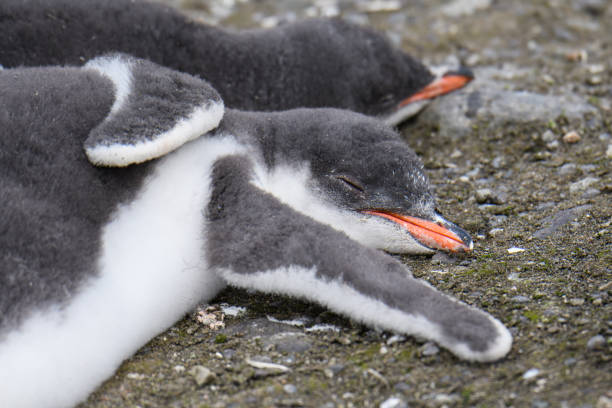
\includegraphics[scale=0.8]{bilder/penguin-sleeping.jpg}

Doch oftmals sollen Bilder flüssig und dynamisch dem Text angepasst werden. Mit der Fließumgebungen \textit{figure} kann hierbei einem Bild eine \textit{caption} und ein \textit{label} gegeben werden. Das Label kann im Text referenziert werden.

\begin{figure}
    
\includegraphics[scale=0.3]{bilder/penguin.png}
    \caption{Ein süßer Pinguin in Fließumgebung}
    \label{fig.pinguin}
\end{figure}

Schaut euch den süßen Pinguin in Abbildung \ref{fig.pinguin} an! Doch warum befindet sich dieser so komisch oben? \LaTeX versucht hier die Abbildung an den restlichen Inhalt der Seite anzupassen und plaziert daher das Bild so komisch an den Anfang. Mit der \textit{[h]} Option der \textit{figure} Fließumgebung kann erzwungen werden, dass die Abbildung an der jetzigen Position eingefügt werden soll. Mit \textit{centering} kann der nachfolgende Inhalt, die Abbildung, zentriert werden.

\begin{figure}[h]
    \centering
    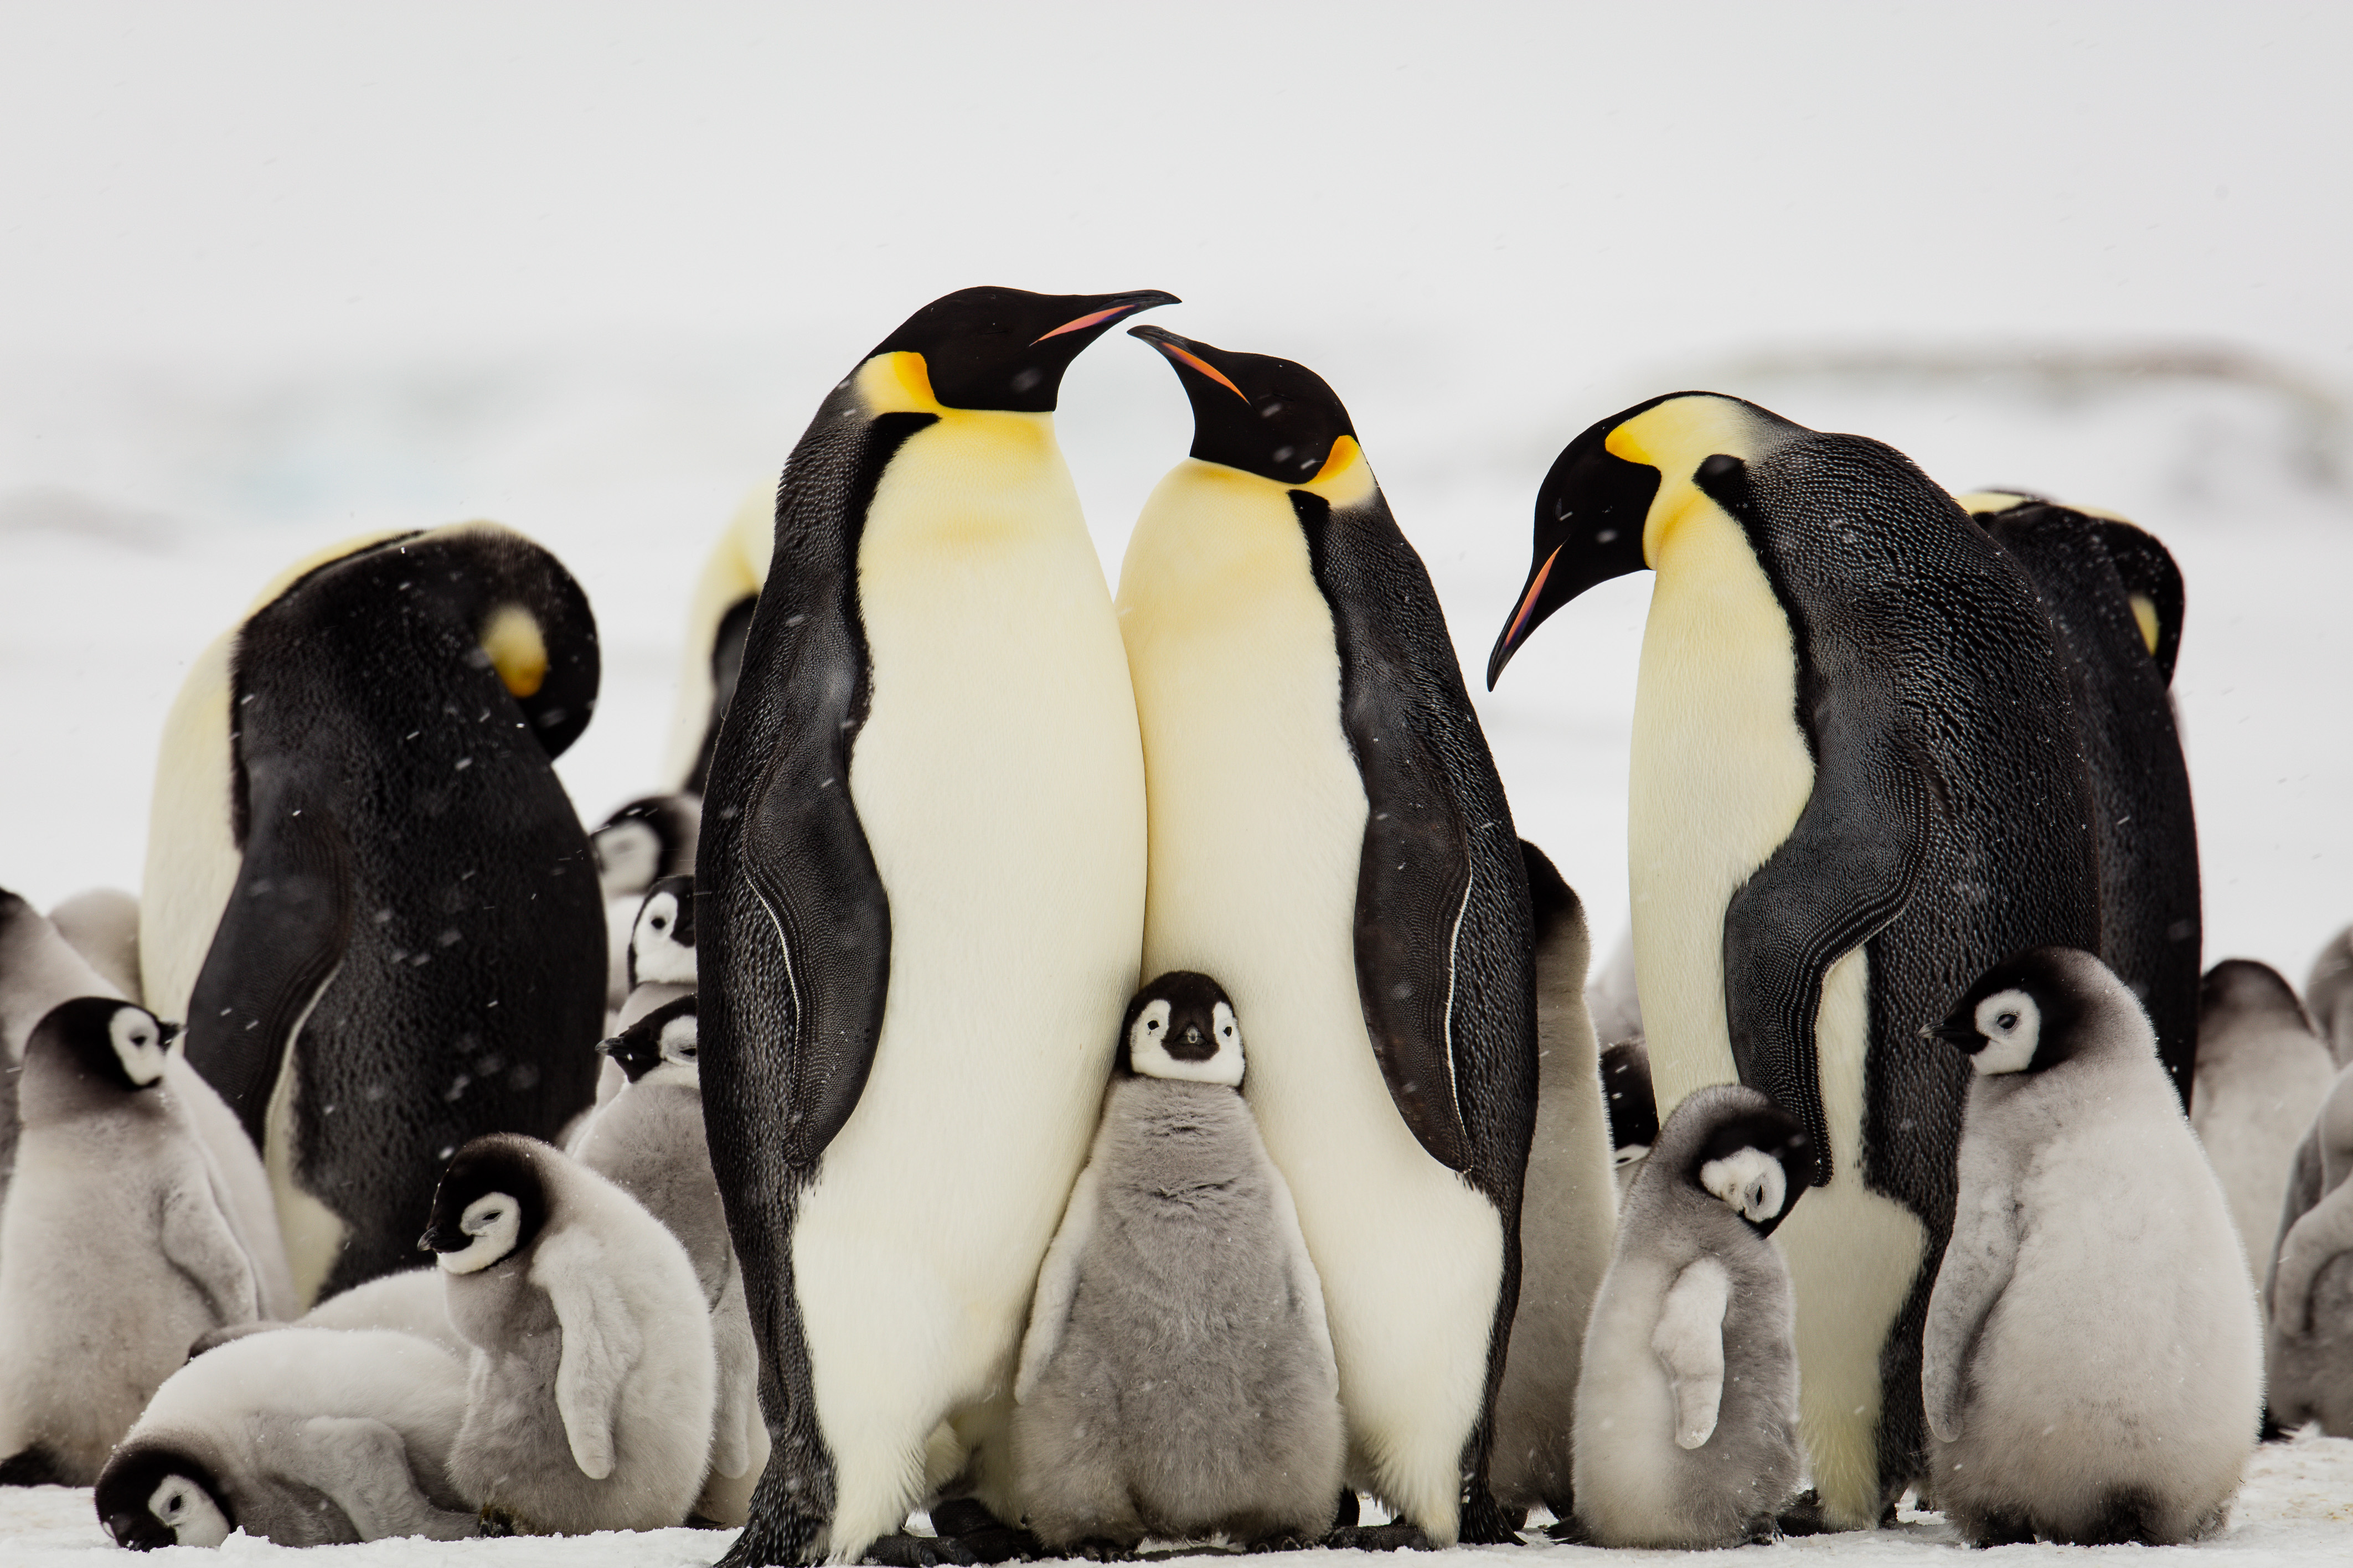
\includegraphics[scale=0.2]{bilder/penguin-family.jpg}
    \caption{Pinguin Familie, awwww}
    \label{fig.pinguinFamily}
\end{figure}

\newpage